\chapter{Anforderungsanalyse}
\label{cha:Anforderungsanalyse}

\autsection{App-Spezifikation}{Mattfeld}
\label{sec:app-spec}
Kurzbeschreibung der App:
\begin{itemize}
\item Darstellung eines Scrum-Boards mit mehreren Spalten
\item Darstellung der Aufgaben in den zugehörigen Spalten
\item Möglichkeit für den User, Aufgaben zwischen den Spalten hin- und herzuschieben
\item Update des Aufgabenstatus  in der Datenbank durch Verschieben
\end{itemize}
\SuperPar
Relevante Backend-Tabellen:
\begin{itemize}
\item zav\_kunden: Kundentabelle
\item zav\_projekte: Projekte je Kunde
\item zav\_sprints: Sprints je Projekt je Kunde
\item zav\_aufgaben: Aufgaben je Projekt, je Kunde, teilweise Sprints zugeordnet
\item zav\_formcust: Definition von Spalten je Projekt je Kunde; Zuordnung von Aufgabenstatus zu Spalten
\end{itemize}


\subsection{Anforderungen}
Die Startsequenz der App ist wie folgt:
\begin{enumerate}
	\item Anmeldung am System
	\item Auswahl eines Kunden
	\item Auswahl eines (zum Kunden gehörigen) Projektes
	\item Auswahl eines (zum Projekt gehörigen) Sprints
	\item Darstellung eines Scrum-Boards mit mehreren Spalten
	\item Darstellung der zu den Spalten gehörigen Aufgaben als Aufgabenzettel
\end{enumerate}
Die Spalten-Überschriften sind dabei dynamisch, jedoch ergibt sich für jedes Projekt ein jeweils eindeutiger Satz an Spalten. Die Einordnung von Aufgaben in den Spalten ergibt sich aus dem Status der Aufgabe; Die Zuordnung von Status-Konstellationen zu Spalten folgt der Tabelle (ZAV\_FORMCUST).

\begin{figure}
	\centering
	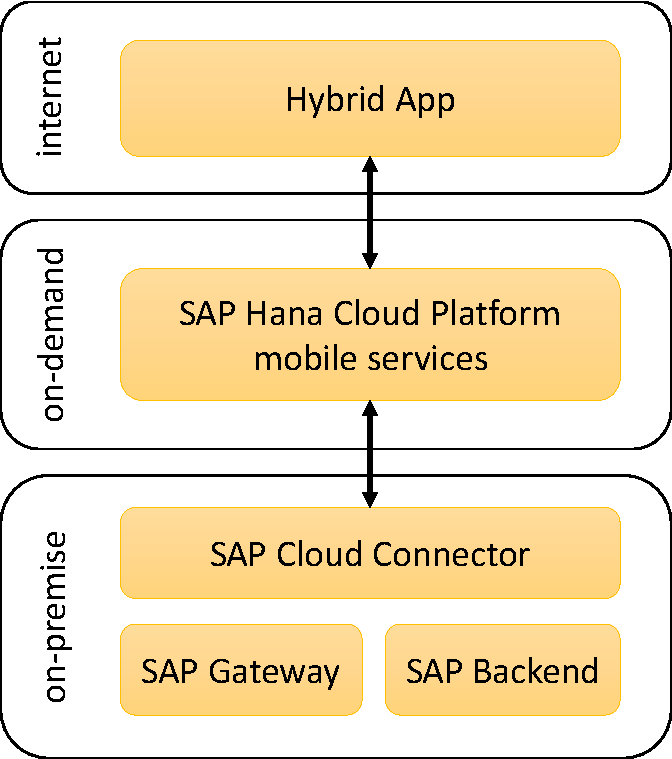
\includegraphics[width=.8\textwidth]{Architektur2} 
	\caption[App-Architektur]{App-Architektur nach \cite{openSAP2014_1}.}
	\label{fig:Architektur2}
\end{figure}

\subsection{Architektur}
\label{sec:app-architektur}
Wie im \autoref{sec:architekturen} beschrieben, gibt es viele Möglichkeiten eine UI5-App zu betreiben und zu veröffentlichen. Die Entscheidung richtet sich nach den benötigten Geräte- und Geschäftsfunktionen sowie der SAP-Integrationstiefe. 

In der ersten Version der Scrum-App sind weder Offline-Funktionen, noch native Gerätezugriffe gefordert. Einzig der Zugriff ohne Intranet-Verbindung erfordert besondere Beachtung. Die empfohlene Lösung ist die Weiterleitung des OData-Services nach außen über die Hana Cloud Platform, siehe \autoref{fig:Architektur2}. Der SAP Cloud Connector stellt die sichere Verbindung zwischen SAP-Backend vor Ort und der Cloud her. Vorteil: Das SAP-Backend des Kunden ist nach außen nicht sichtbar, die Firewall-Konfiguration muss nicht angepasst werden. App-Benutzer melden sich direkt an der Cloud-Plattform an, benötigen also keinen Intranet-Zugriff per VPN mehr.


%\subsection{Aufwandsschätzung}


\section{Testkonzept}
Das Testkonzept orientiert sich an IEEE\,829 \cite{IEEE829}, angepasst an die kleinere Projektgröße. Es ist als Dokument für alle Aktivitäten während des gesamten Projekts gültig. Darüber hinaus soll es als Vorlage für zukünftige App-Entwicklungen dienen. Ziel ist die Umsetzung des fundamentalen Testprozesses nach Spillner \cite{SpillnerRossnerWinterLinz2014}. In anderen Teilen der Arbeit behandelte Testwerkzeuge werden nicht beschrieben. Berücksichtigt werden folgende Dokumente:
\begin{itemize}
	\item Anforderungsspezifikation des Kunden, siehe \autoref{sec:app-spec}
	\item UI5 Development Conventions and Guidelines \cite{SAP2014_1}, insbesondere:
	\begin{itemize}
		\item JavaScript Coding Guidelines
		\item UI5 Control Development Guidelines
		\item Product Standards/Acceptance Criteria
		\item Git Guidelines
		\item File Names and Encoding	
	\end{itemize}
	\item SAP Gateway Best Practices (\cite[S.\ 561-563]{BoennenDreesFischerHeinzStrothmann2014})
	\item Projektvorgehen: Testgetrieben inkl. \ac{CI} (siehe \autoref{cha:Grundlagen})
\end{itemize}


\subsubsection{Testobjekte}
Der Architektur aus \autoref{sec:app-architektur} folgend, besteht die Anwendung aus zwei Hauptkomponenten. Beide sind Teil des Testkonzepts:
\begin{itemize}
	\item HTML5-Frontend (OpenUI5 1.26.8)
	\item SAP-Backend
	\begin{itemize}
		\item Funktionsbausteine (ECC 6.0, EHP 7, NW 7.4)
		\item OData-Service (SAP Gateway NW 7.4)
	\end{itemize}
\end{itemize}
Nicht einzeln getestet werden die JavaScript-Frameworks wie OpenUI5 und die verwendeten Test-Frameworks. Die Testbasis der entsprechenden Open-Source-Projekte ist mit diversen Unit- und Akzeptanztests sehr umfangreich. Eine projektinterne Test-Wiederholung bringt keinen Mehrwert.


\autsubsection{Steuerung und Planung}{Mattfeld}
Durch die kleine Teamgröße sind Entwickler gleichzeitig Tester (Test-Manager, Designer, Automatisierer, \dots).
Sie erarbeiten gemeinsam mit dem Kunden nach dem Prinzip des \ac{BDD} allgemein verständliche Anforderungen. Die Beschreibung der Fallbeispiele erfolgt im Schema von automatisierbaren \textit{Wenn-Dann}-Sätzen.

Fehlerkosten verdoppeln sich in jeder Entwicklungsphase. Der Kunde wird daher besonders stark in die Designphase einbezogen, um Kosten durch späte Änderungen zu vermeiden.

\subsubsection{Risiko und Kosten}
Insgesamt sind Fehlerkosten schwer abzuschätzen. Schadenshöhe und Wahrscheinlichkeit sind durch interne, ergänzende Verwendung der App überschaubar: Die Scrum-Aufgaben werden nur angeschaut oder im Status verändert. Nutzereingaben über den Client müssen allerdings immer als kritisch eingestuft werden. Gültigkeitsprüfungen in der App dienen nur der schnellen Rückmeldung an den User und Trafficvermeidung, nicht der Sicherheit. Das Backend ist daher ausführlich zu betrachten. 

Durch eine Fehlfunktion besteht eine Gefahr für laufende Projekte bei diversen Kunden. Daraus folgen direkte Schäden und Imageverlust. Fehlerkorrekturkosten werden durch TDD und CI eingegrenzt -- Regressionstests und Deployment sind automatisiert.

Testkosten sind ebenso schwierig vorauszusehen. Vor allem der geringe Reifegrad des Entwicklungsprozesses erschwert die Schätzung: Bisherige Erfahrungen sind durch den prototypischen Projekt-Charakter nicht vorhanden. Der Testplan kommt zum ersten Mal zum Einsatz. Allerdings wird die Testbarkeit und Modularität der Software durch testgetriebene Entwicklung sichergestellt. Zusätzlich ist die Testinfrastruktur von Anfang an vorhanden und erfüllt alle Anforderungen an Continous Integration. Die Projektteilnehmer sind mit diesen Werkzeugen vertraut und beherrschen die Grundlagen des Testens nach ISTQB.

Die höchste Priorität haben die Tests des sicherheitskritischen Backends. In der App-Komponente decken die Akzeptanzkriterien Funktionalitäten mit hoher Nutzungshäufigkeit ab. Sie stehen im Mittelpunkt der Kundenwahrnehmung des Produktes und werden entsprechend wichtig eingestuft. 

Testaufwand: Eine vollständige Analyse der Aufwände ist nicht möglich und Erfahrungswerte sind noch nicht vorhanden. Diese Herausforderungen stellen ein großes Projektrisiko dar. Zumindest durch bekannte QM-Werkzeuge und hohe Automatisierung soll die Erfolgswahrscheinlichkeit erhöht werden. Den Testaufwand schätzen wir bei diesem Prototypen mit mindestens 50\,\% des Gesamtentwicklungsaufwands ein.

\subsubsection{Qualitätsziele und Testabedeckung}
Testendkriterium ist eine Anforderungsüberdeckung von 100\,\%. Ebenso müssen die sicherheitskritischen Äquivalenzklassentests des Backends zu 100\,\%. erfolgreich laufen. Testabbruchkriterien sind fehlgeschlagene Unit- und Akzeptanztests. Fehler der statischen Analyse führen ebenso zum Abbruch, Warnungen oder Schwankungen in den Komplexitäts-Metriken allerdings nicht.

Die nicht-funktionalen Anforderungen des UI5-Design-Guides können nur teilweise durch statische Analysen automatisiert überprüft werden. Gezielte Reviews während der Designphase und bei größeren Änderungen ergänzen die automatische Analyse. Die Performance der App wird im Rahmen der Systemtests überprüft. Die Akzeptanztests werden hierzu mit kurzen Timeouts angepasst.

\subsubsection{Konfigurationsverwaltung}
Die Konfigurationsverwaltung erfolgt per Git über die Plattform GitHub. Es gelten die UI5 Guidlines zu Git Commits: Es muss jederzeit nachvollziehbar sein, wer, wann, warum, welche Codezeilen geändert hat.

Eingecheckt wird nicht nur der Programmcode, sondern auch die Dokumentation, Tests und die CI-Toolchain. Das Prinzip \textit{Infrastructure as a Code} ist vollständig umgesetzt. Das bedeutet, die gesamte Build- und Deployment-Umgebung kann auf einem neuen System automatisch wiederhergestellt werden. 

Die Abhängigkeiten der Tool- und Framework-Versionen sind in Konfigurationsdateien hinterlegt und werden über die Paketmanager aufgelöst. Über Git werden Zwischenversionen der App gekennzeichnet oder in Branches ausgegliedert. Die Wiederherstellung eines bestimmten Entwicklungsschrittes inklusive Dokumentation, Buildumgebung und Tests ist stets gewährleistet. 

Das CI-System stellt die Gültigkeit der Konfigurationsverwaltung sicher. Jede Neuerung in der Versionskontrolle löst einen vollständigen Neuaufbau der Buildumgebung auf dem CI-Server anhand der Konfiguration aus.


\subsubsection{Fehlermanagement}
Ein Testprotokoll wird für jeden Build separat auf dem CI-Server vorgehalten. Das gesamte Projektteam hat Zugriff auf das Protokoll. Zusätzlich wird der Build-Status im Repository visualisiert. Das Team ist jederzeit über den Teststatus informiert.

Durch \ac{TDD} existiert theoretisch kein ungetesteter Code. Die QA-Pipeline wird in einem \textit{Private Build} auf dem Entwicklungsrechner komplett durchlaufen. Noch nicht implementierte Funktionalitäten bzw. die zugehörigen roten Tests werden auch nicht in die globale Versionsverwaltung eingecheckt. Neue Fehlerwirkungen werden vor allem während der höheren Teststufen wie Integrations-, System- und Akzeptanztests auftreten. Denkbar sind auch Inkompatibilitäten mit Browsern und Endgeräten oder Probleme mit dem CI-Prozess selbst.

 Da alle Projektartefakte in der Versionsverwaltung eingecheckt werden, ist auch das Fehlermanagement zentral für alle Projektteilnehmer. Das Schema einer Fehlermeldung ist festgelegt und beinhaltet eine eindeutige Fehlernummer, Entdecker, Erfassung und Problembeschreibung. Angaben zur zugehörigen Anforderung, Fehlerquelle und Reproduktion werden wenn möglich eingetragen. Über verschiedene Labels werden für dieses Projekt individuell gesetzt: Fehlerklasse (Bug, Enhancement, Documentation), Priorität (open, wontfix) und Status (new, open, approved, invalid, question, duplicate, works, fixed).

Testfälle und Korrekturen werden über einen Fork eingebracht. Beides kann per Kommentarfunktion diskutiert werden. Ist der Fehler durch einen Testfall nachgewiesen und die Code-Korrektur akzeptiert, schließt ein Kommentar im Commit automatisch das Issue Ticket.

%\subsection{Design und Analyse}
%Testbasis prüfen (Anforderungen), Testbarkeit prüfen, Logische Testfälle

\subsection{Durchführung}
\label{sec:tests}
Die Testfälle unterteilen sich in verschiedene Teststufen:
\begin{itemize}
	\item Komponententests der Funktionsbausteine
	\item Integrationstests zwischen Backend und Gateway
	\item Isolierter Akzeptanztests der App mit Mockserver
	\item Systemtest mit App und Gateway
\end{itemize}

\subsubsection{Akzeptanztest-Szenario 1: Kundenübersicht}

\textbf{Given} I start the app\\
\textbf{When} I look at the screen\\
\textbf{Then} I should see the customer list\\
\textit{and} the customer list should have entries\\

\subsubsection{Akzeptanztest-Szenario 2: Projektübersicht}

\textbf{Given} I start the app\\
\textbf{When} I press on customer 1\\
\textbf{Then} I should be taken to customer 1\\
\textit{and} I should see the project list of customer 1\\
\textit{and} the project list should have entries\\



\subsubsection{Äquivalenzklassentest}
Um alle möglichen Eingabewerte für einen Funktionsbaustein zu ermitteln, werden Äquivalenzklassen für die jeweiligen Eingabeparameter gebildet, siehe \autoref{tab:aquivalenzklassen-FubaProjekte}. Hierbei ist darauf zu achten, dass für jeden Parameter auch negative Werte getestet werden. Da die Anzahl der Testfälle bei einfacher Multiplikation der möglichen Kombinationen schnell zu einer erheblichen Anzahl ansteigt, werden gültige Äquivalenzklassen in den Testfällen kombiniert. Ungültige Äquivalenzklassen dürfen wiederum nur mit gültigen Äquivalenzklassen kombiniert werden, sodass für jede ungültige Äquivalenzklasse ein eigener Testfall erstellt wird \cite[S.\ 110-115]{Spillner2010}. Die daraus entstandenen Testfälle sind in \autoref{tab:test-read-projektet} zu sehen. Damit wird eine Äquivalenzklassenüberdeckung von 100\,\% für den zu testenden Funktionsbaustein erreicht.

\begin{table}[h]
	\centering
\begin{tabular}{cccc}
	\toprule Äquivalenzklasse & Parameter & Eingabewert & ÄK gültig?\\
	\midrule ÄK1 & Kunde  & ''TKMI''  & Ja\\ 
			ÄK2 & Kunde & ''tkmi'' & Nein\\
			ÄK3 & Kunde & - & Nein\\
			\midrule
			ÄK4 & Projekt & ''TM-SCRUM'' & Ja\\
			ÄK5 & Projekt & ''tm-scrum'' & Nein\\
			ÄK6 & Projekt & - & Ja\\
			\midrule
			ÄK7 & Substring & ''TM-SCRUM'' & Ja\\
			ÄK8 & Substring & ''tm-scrum'' & Ja\\
			ÄK9 & Substring & ''asdf'' & Nein\\
			ÄK10 & Substring & - & Ja\\
			\midrule
			ÄK11 & Projekt und Substring & nicht leer & Nein\\
	\bottomrule 
\end{tabular} 
\caption{Äquivalenzklassen für den Funktionsbaustein Z\_SCRUMUI5\_READ\_PROJEKTE}
\label{tab:aquivalenzklassen-FubaProjekte}
\end{table} 

\begin{table}[h]
	\centering
\begin{tabular}{cccccc}
	\toprule Testfall & getestete ÄK & Kunde 	& Projekt 		& Substring 	&  Ergebnis \\ 
	\midrule     1 	 &  1,6,10 		& ''TKMI'' 	& - 			& - 			&  Anzeige erfolgt\\ 
			 2 	 & 4			& ''TKMI'' 	&''TM-SCRUM'' & - 			& Anzeige erfolgt\\ 
			 3	 &  7			& ''TKMI'' 	& - 			& ''TM-SCRUM'' & Anzeige erfolgt\\ 
			 4	 &  8			& ''TKMI'' 	& - 			& ''tm-scrum''	& Anzeige erfolgt\\ 
			5 	 &  2			& ''tkmi'' 	& - 			& - 			& Keine Anzeige\\ 
			6 	 &  3			& - 		& - 			& - 			& Keine Anzeige\\ 
			7 	 &  5			& ''TKMI'' 	& ''tm-scrum''	& - 			& Keine Anzeige\\ 
			8 	 &  9			& ''TKMI'' 	& - 			& ''asdf'' 		& Keine Anzeige\\ 
			 9 	 & 11			& ''TKMI'' 	& ''TM-SCRUM''	& 'TM-SCRUM''		& Keine Anzeige\\ 
	\bottomrule 
\end{tabular} 
\caption{Ermittelte Testfälle für den Funktionsbaustein Z\_SCRUMUI5\_READ\_PROJEKTE}
\label{tab:test-read-projektet}
\end{table} 

%Äquivalenzklassen-Überdeckung = (Anzahl getesteter ÄK / Gesamtanzahl ÄK) x 100\%

\subsubsection{Testfälle OData-Service}
Die relevanten Testfälle (siehe \autoref{tab:testfälle-OData}) für den OData-Service werden durch die verwendeten OData-Funktionen bestimmt. Dabei ist zwischen den allgemeinen Testfällen für den kompletten OData-Service, sowie den Funktionen die für jede Entität einzeln getestet werden zu unterscheiden.

\begin{table}[h]
	\centering
\begin{tabular}{ccccc}
	\toprule Testfall & OData-Funktion  \\
	\midrule 	
	Allgemeine Testfälle: & \\
	\midrule
	TF1 & JSON-Format \\
	 	    	TF2 & Servicedokument \\
			TF3 & \$metadata\\
	\midrule
	Testfälle je Entität: & \\
	\midrule		
			TF4 & \$expand\\
			TF5 & Navigation\\
			TF6 & Navigation mit \$links\\
			TF7 & \$count \\
			TF8 & \$ordberby\\
			TF9 & \$skip\\
			TF10 & \$top\\
			TF11 & GetEntititySet\\
			TF12 & GetEntitity\\
			TF13 & \$filter\\
	\bottomrule 
\end{tabular} 
\caption{Testfälle - OData-Service}
\label{tab:testfälle-OData}
\end{table} 
